\xiaosi

为展示NCP相比黑箱模型的可解释性优势，本节从参数效率和结构可解释性两个维度进行分析。

\subsubsection{参数效率分析}

图\ref{fig:pareto}展示了各模型在highway-v0上的参数量-性能帕累托前沿。NCP位于左上角（少参数、高性能），是帕累托最优点。具体而言，NCP的参数效率（reward/千参数）为4.89，是MLP（2.64）的1.9倍，GRU（1.63）的3.0倍，LSTM（0.94）的5.2倍。这说明NCP的生物启发稀疏结构能够以极高的参数利用率编码驾驶策略。

\begin{figure}[H]
    \centering
    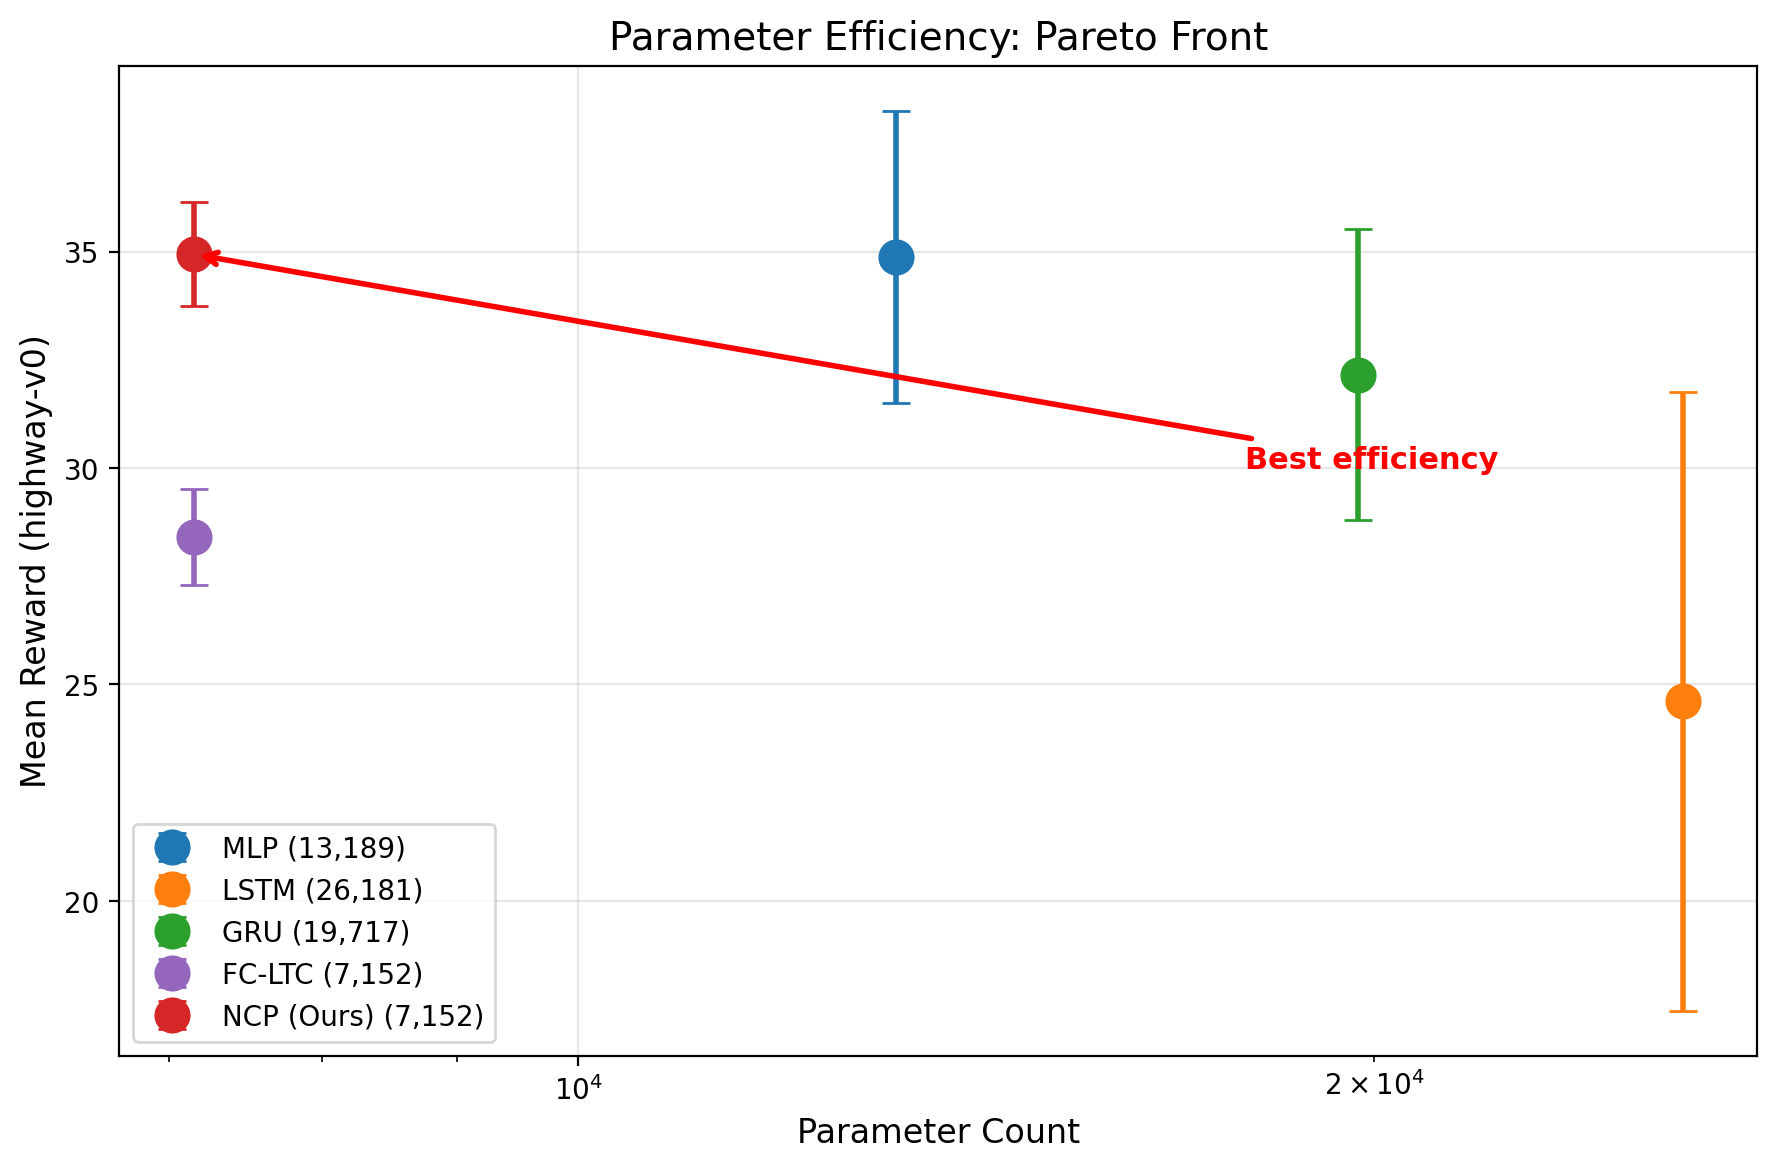
\includegraphics[width=0.75\linewidth]{img/fig_pareto_front.png}
    \caption{参数量与性能的帕累托前沿图（highway-v0场景）}
    \label{fig:pareto}
\end{figure}

\subsubsection{命令神经元激活分析}

图\ref{fig:activations}展示了一次highway-v0完整episode中8个命令神经元的激活值（热图），以及同步的Q值曲线、动作序列和奖励。可以观察到：（1）不同命令神经元呈现明显不同的激活模式——Cmd 3和Cmd 7持续高激活（深红），Cmd 4为强负激活（深蓝），说明各神经元承担了差异化的功能角色；（2）在动作切换时刻（如第5-7步从IDLE切换到SLOWER再到RIGHT），命令层激活发生同步跃变，表明命令层确实编码了决策信号。

\begin{figure}[H]
    \centering
    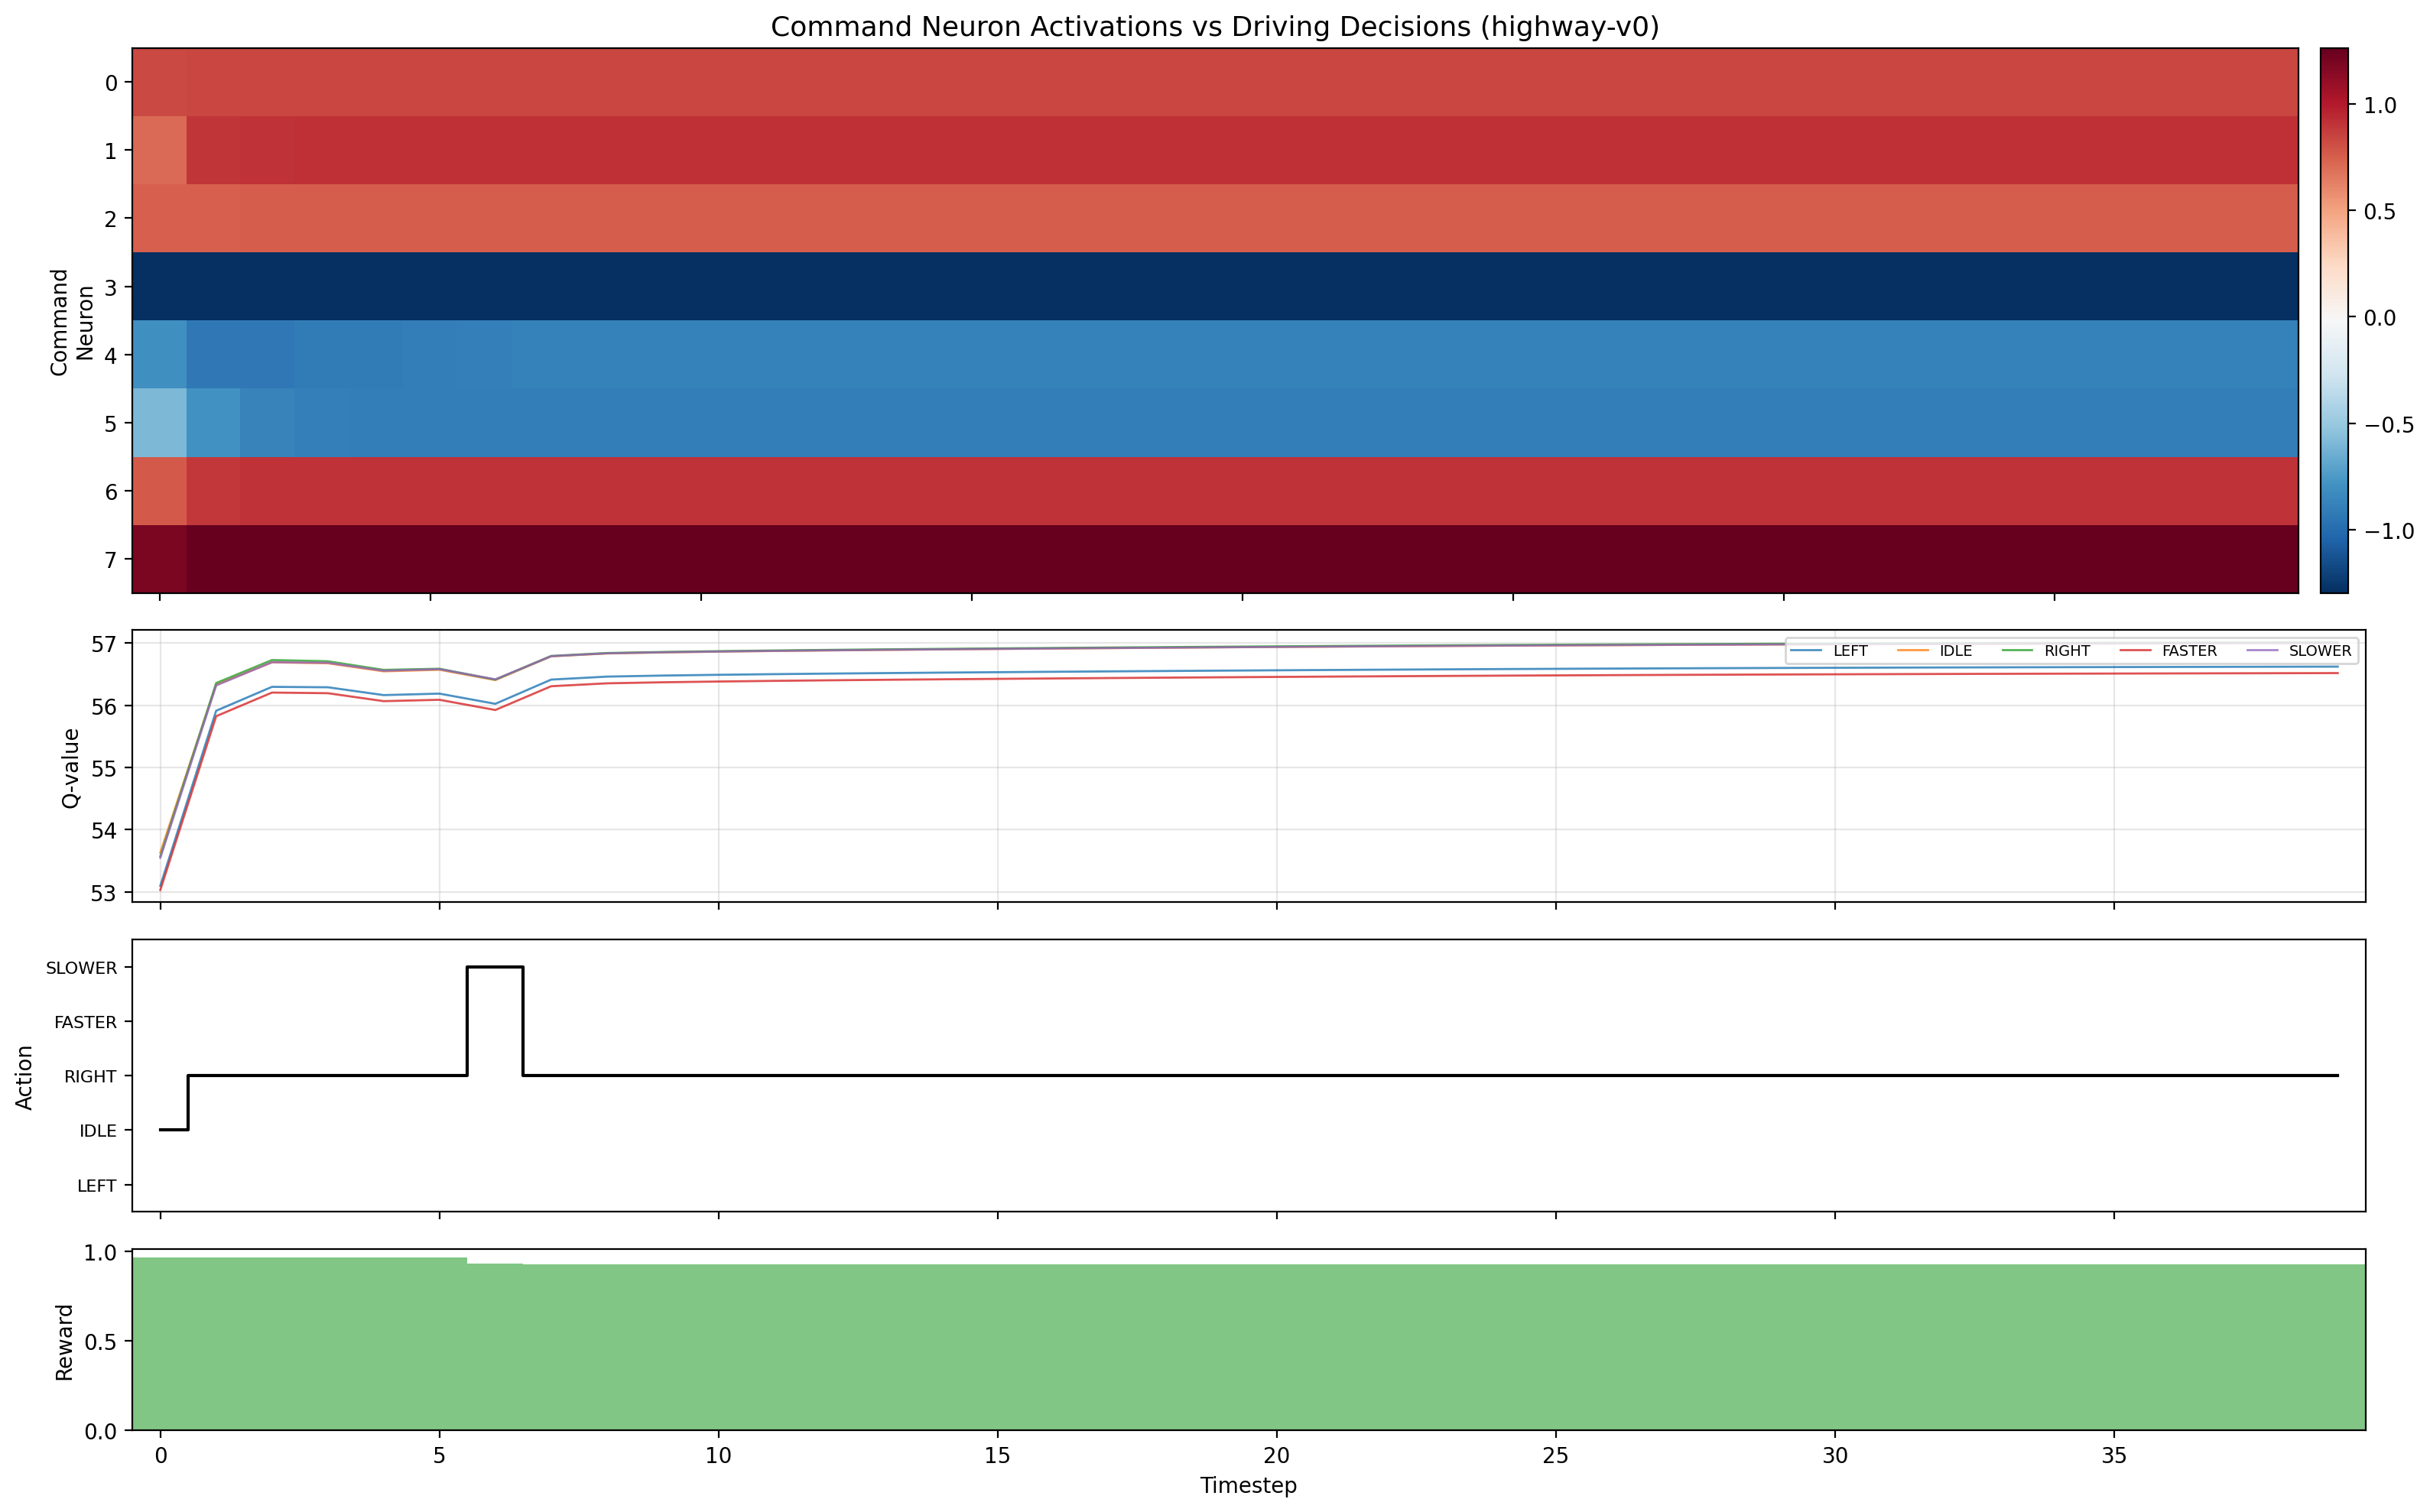
\includegraphics[width=1.0\linewidth]{img/fig_activations_highway.png}
    \caption{highway-v0场景中命令神经元激活、Q值、动作和奖励的时序对齐图}
    \label{fig:activations}
\end{figure}

\subsubsection{神经元功能归因}

为定量分析每个命令神经元对各动作的影响，本文采用逐神经元mask实验：依次将每个命令神经元的激活置零，测量Q值的变化量$|\Delta Q|$。图\ref{fig:attribution}展示了归因矩阵。

Cmd 7对所有动作影响最大（$|\Delta Q|$达2.96--3.17），是最关键的全局决策神经元；Cmd 1影响最小（约1.0），可能是冗余神经元。值得注意的是，Cmd 0对LEFT动作的影响（2.40）明显高于对RIGHT的影响（2.07），暗示该神经元编码了方向选择性信息。

\begin{figure}[H]
    \centering
    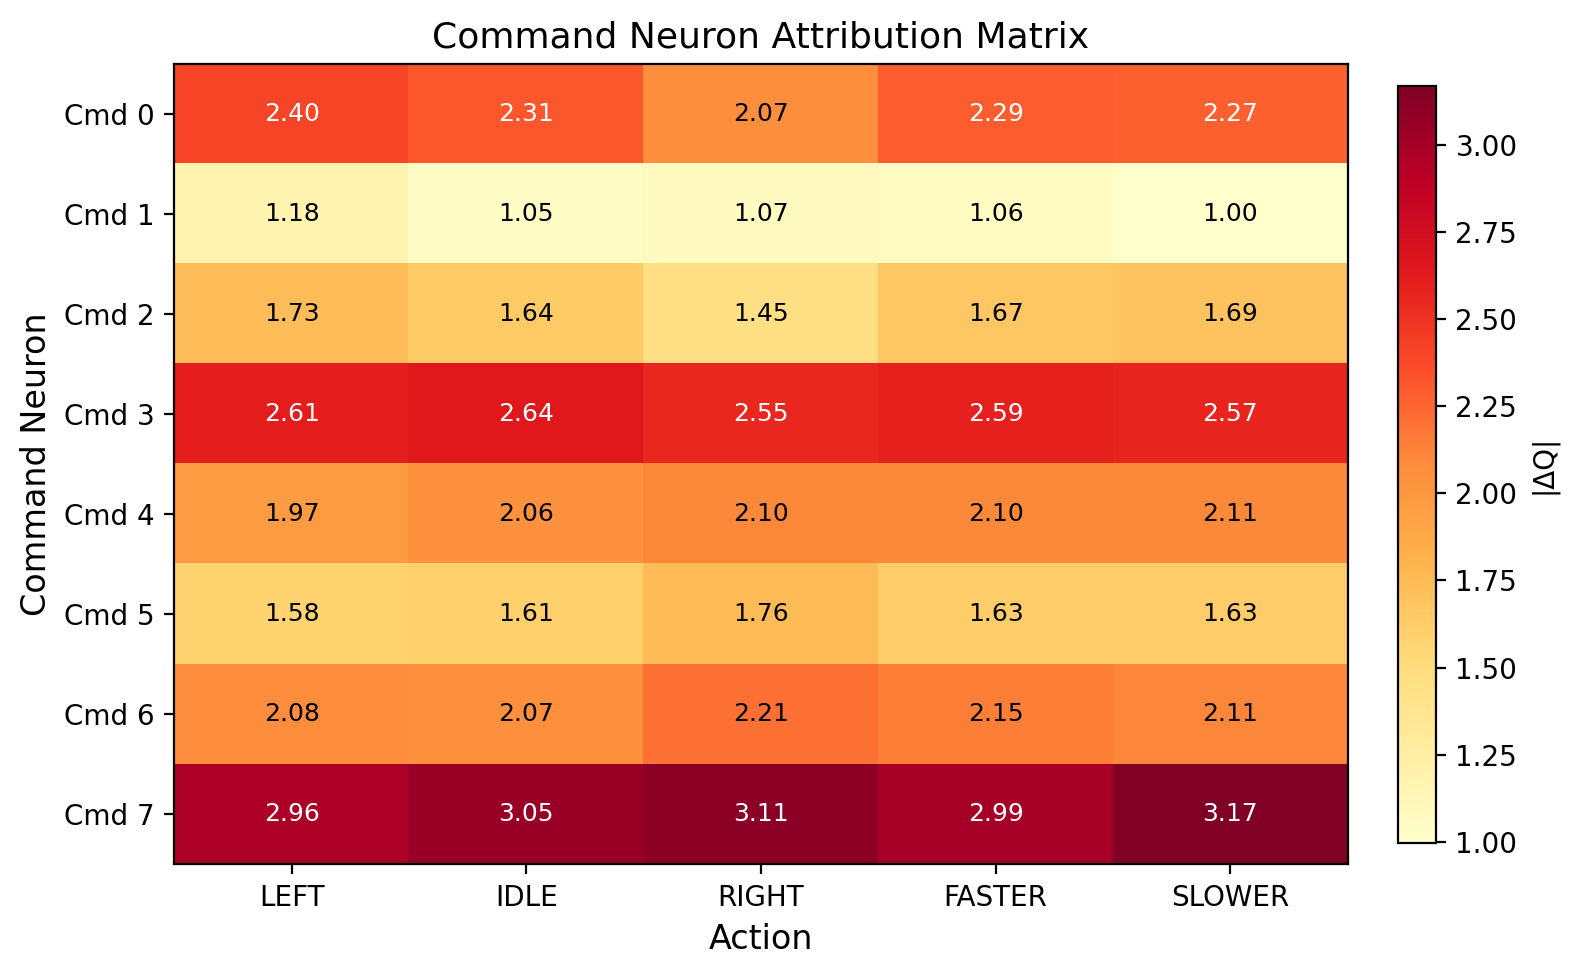
\includegraphics[width=0.75\linewidth]{img/fig_neuron_attribution.png}
    \caption{命令神经元功能归因矩阵（逐神经元mask后Q值变化量）}
    \label{fig:attribution}
\end{figure}

\subsubsection{跨场景激活模式对比}

图\ref{fig:pca}展示了4个驾驶场景下命令层激活的PCA降维结果。前两个主成分解释了84.6\%的方差（PC1: 47.6\%, PC2: 37.0\%）。Highway场景的激活点分布最广（episode最长），Intersection和Roundabout的点较分散（场景复杂度高），且4个场景在PCA空间中存在部分重叠——这说明NCP学到了一些场景无关的通用决策模式（如减速避障），同时也能区分不同场景的特有状态。

\begin{figure}[H]
    \centering
    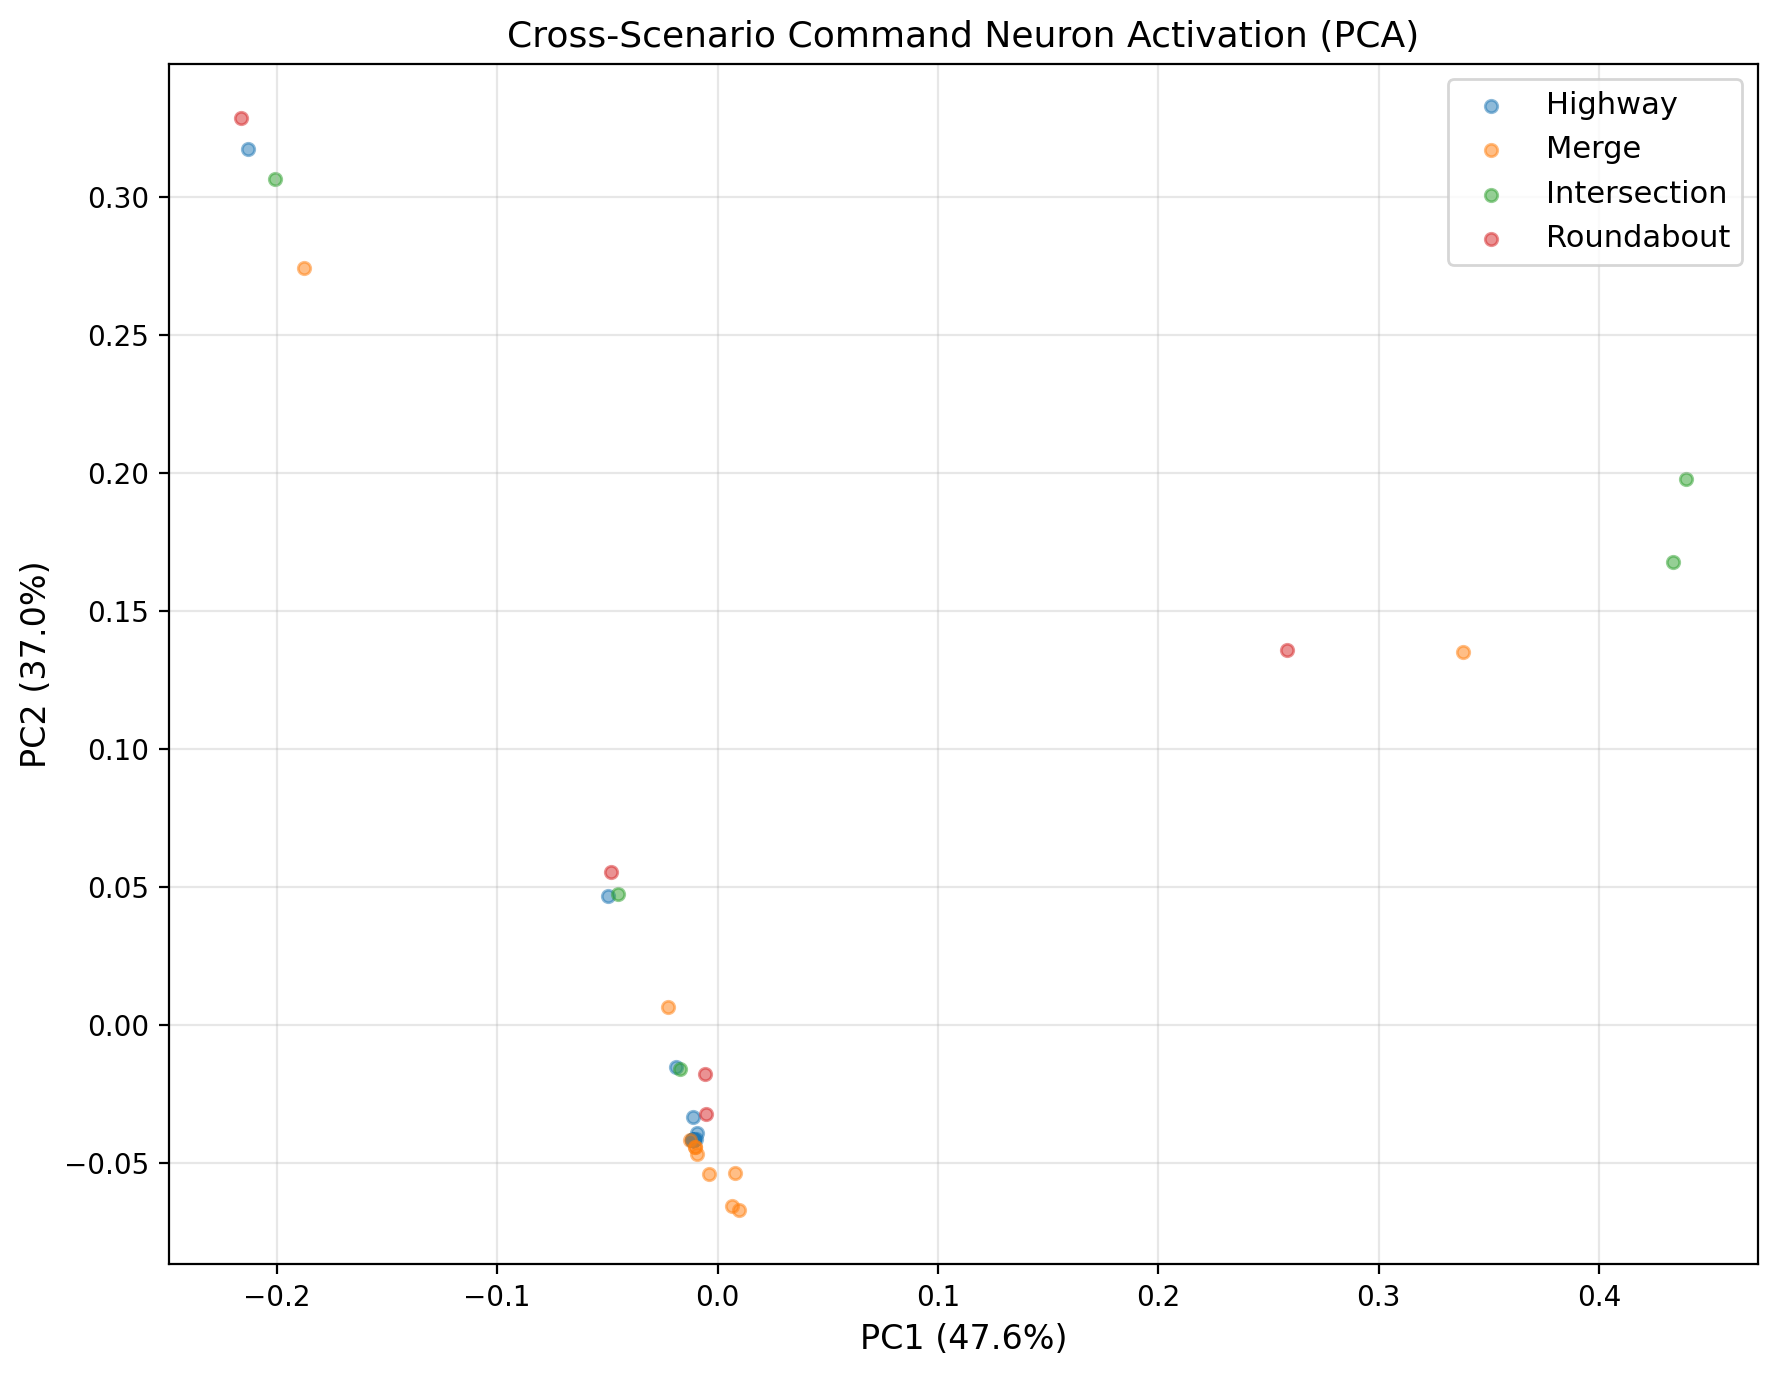
\includegraphics[width=0.7\linewidth]{img/fig_activation_pca.png}
    \caption{4个驾驶场景下命令神经元激活的PCA降维可视化}
    \label{fig:pca}
\end{figure}

\subsubsection{结构可解释性讨论}

NCP的可解释性优势源于其结构化设计，具体体现在三个层面：

\textbf{层次化功能分工。}四层布线使感觉层、中间层、命令层、运动层各司其职。感觉层编码环境特征，中间层整合信息，命令层做出决策，运动层输出控制——信息流路径可被完整追踪。对比之下，MLP和LSTM的全连接结构中，任何一个隐藏单元都可能同时参与编码、整合和决策，难以分辨各单元的功能角色。

\textbf{兴奋/抑制极性。}NCP的每条突触具有明确的兴奋性（$+1$）或抑制性（$-1$）标签，提供了因果推理线索。例如，一条从命令层到运动层的抑制性连接可以被解读为"该命令神经元抑制了某个动作的选择"。这种内置的因果结构是传统神经网络所不具备的。

\textbf{可审计的规模。}默认NCP仅25个神经元，搜索出的拓扑更是只有15个。这使得对网络进行逐神经元审计成为可能——人类可以检查每个神经元在特定决策中的角色。相比之下，LSTM的64维隐藏状态和MLP的128维中间层远超人类直接理解的能力。

以上三个层面的可解释性是NCP的内在属性，无需额外的事后解释方法（如Grad-CAM），且在拓扑搜索后仍然保持——搜索出的15神经元拓扑同样具备完整的层次分工和极性标注。这为自动驾驶系统满足欧盟AI法案的透明性要求\cite{euaiact2025}提供了结构性支撑。
